En este último curso se ha profundizado intensamente sobre la calidad del
producto y se han usado algunas herramientas para comprobar objetivamente la
calidad del mismo. En esta sección se tratarán las herramientas usadas para
validar el proyecto de forma objetiva.

\subsection{Lighthouse}\label{lighthouse}
Lighthouse es una herramienta automatizada de código abierto para mejorar el
rendimiento, la calidad y la corrección de sus aplicaciones web.

Al auditar una página, Lighthouse ejecuta un aluvión de pruebas contra la
página y luego genera un informe sobre qué tan bien lo hizo la página. Desde
aquí puede utilizar las pruebas de falla como indicadores de lo que puede hacer
para mejorar su aplicación.\cite{lighthouse-resume}

\begin{figure}[htb!]
    \centering
    \caption{Logo de Lighthouse} \label{fig:lighthouse-logo}
    \centering
    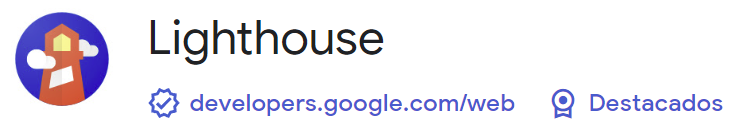
\includegraphics[scale=0.35]{./Ilustraciones/logos/lighthouse-logo.png}\\
    \textbf{Fuente:} Chrome Web Store [\url{https://chrome.google.com/webstore/detail/lighthouse/blipmdconlkpinefehnmjammfjpmpbjk?hl=es}]
\end{figure}

Con esta herramienta se pretende obtener objetivamente una versión más
accesible de la aplicación, que los colores tengan una coherencia, sean
visibles de una forma correcta sin constrastes extraños o disonancias de tonos,
así como una ayuda a la hora de controlar el SEO de la aplicación.

\subsection{SonarQube}\label{sonarqube}
SonarQube es una herramienta de revisión de código automática y autogestionada
que ayuda sistemáticamente a entregar código limpio. SonarQube se integra en su
flujo de trabajo existente y detecta problemas en su código para ayudarlo a
realizar inspecciones continuas de código de sus proyectos. La herramienta
analiza 30+ lenguajes de programación diferentes y se integra en su
canalización de CI y plataforma DevOps para garantizar que su código cumpla con
los estándares de alta calidad\cite{sonarqube-resume}.

\begin{figure}[htb!]
    \centering
    \caption{Ciclo que propone SonarQube} \label{fig:sonar-cicle}
    \centering
    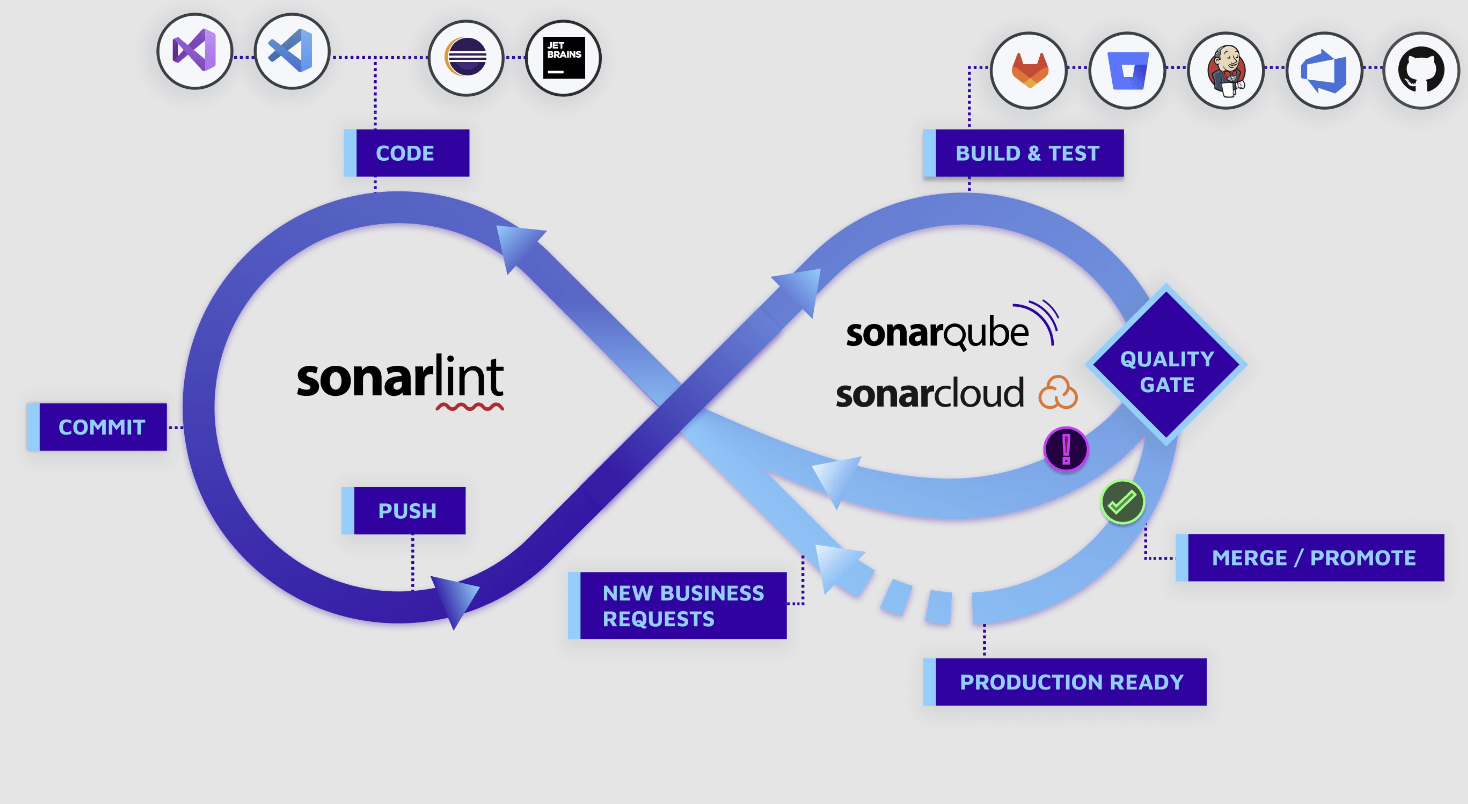
\includegraphics[scale=0.3]{./Ilustraciones/sonarqube.png}\\
    \textbf{Fuente:} Página oficial de SonarQube \url{https://docs.sonarqube.org/latest/}
\end{figure}

Con esta herramienta se pretende llegar a tener la menor cantidad de Code
Smells\footnote{El \textbf{code smell} es una indicación de la mala calidad del
código. Si hay code smells, quien lea el código tendrá la sensación de que algo
está mal. Este se soluciona refactorizando código.[\cite{code-smell}]}
posibles, así como que la deuda técnica\footnote{La \textbf{deuda técnica} es
    el costo del retrabajo adicional causado por la elección de la solución más
    rápida en lugar de la más efectiva.\cite{deuda-tecnica}} sea la menor posible.
También evitar la aparición de bugs, o vulnerabildiades en el código.